% Slide bodies of translation_appendix.tex. Numbers: docs/flow/translation/*.csv;
% tables/*.tex are written by scripts/flow/translation_tables.py.

% ---------------------------------------------------------------- T1
\begin{frame}{Appendix: unpaired PYTHIA $\to$ JEWEL jet translation, a first pilot}
\small
\textbf{Question.} Can the existing unpaired methods map a \emph{clean} PYTHIA jet image to an output with
held-out JEWEL statistics while keeping a meaningful dependence on the input jet? There is no matched JEWEL jet
per PYTHIA jet: any unpaired map is one choice among many with the same marginals. Nothing here is a per-event
medium modification.

\vspace{0.2em}
\begin{columns}[T]
\column{0.5\textwidth}
\footnotesize
\textbf{Data} (own caches, splits, normalisation)
\begin{itemize}\setlength\itemsep{0.0em}
\item parents = (generator file, event): PYTHIA 2.64M, JEWEL 870k clean images; 7.2\% of the PYTHIA images
  are exact copies across files, dropped
\item one leading jet per parent, the closure's code for both: cone $\ge$ 10 GeV, axis $|\eta| < 0.73$, the
  53 R = 0.4 towers in GeV on 16 $\times$ 16; no per-jet normalisation
\item by parent: PYTHIA 200k / 10k / 20k, JEWEL 200k / 10k / 20k + 20k ref; the old JEWEL test jets reserved
\item the crop drops half the event energy (out-of-cone radiation, recoil, the other jet)
\item PYTHIA's cone $E$ starts near 20 GeV, JEWEL's at 10: generators and selections differ, not only the
  medium
\end{itemize}
\column{0.5\textwidth}
\footnotesize
\textbf{Models} (seed 0, UVCGAN-S backbone, 2 A6000 GPU h each, final checkpoint)
\begin{itemize}\setlength\itemsep{0.0em}
\item \ot{}: exact minibatch OT (256), squared $L^2$ of the standardised $\log(E + 0.1)$ canvases, straight
  path; ODE midpoint, NFE fixed on validation (128); 4 Euler$^\ast$: speed only
\item \dsbm{}: independent-pair bridge 0.5 h, online refinement 1.5 h (rollouts in the budget),
  $\varepsilon = 0.25$, SDE 30 steps; one sample per jet (8 on 1000 jets)
\item no new backbone, conditioning, shape or conservation loss, sweep, or test-data choice
\end{itemize}
\textbf{Baselines:} identity (the PYTHIA jet); random JEWEL (training jets, input ignored); JEWEL ref (held-out
JEWEL: the finite-sample floor).\\
\textbf{Read-out fixed before training:} W1 to JEWEL test with bootstrap errors, input correlations,
own-input preference, artefact flags.
\end{columns}
\end{frame}

% ---------------------------------------------------------------- T2
\begin{frame}{Distributions: \ot{} at the JEWEL-vs-JEWEL floor, \dsbm{} halfway}
\vspace{-0.9em}
\begin{center}
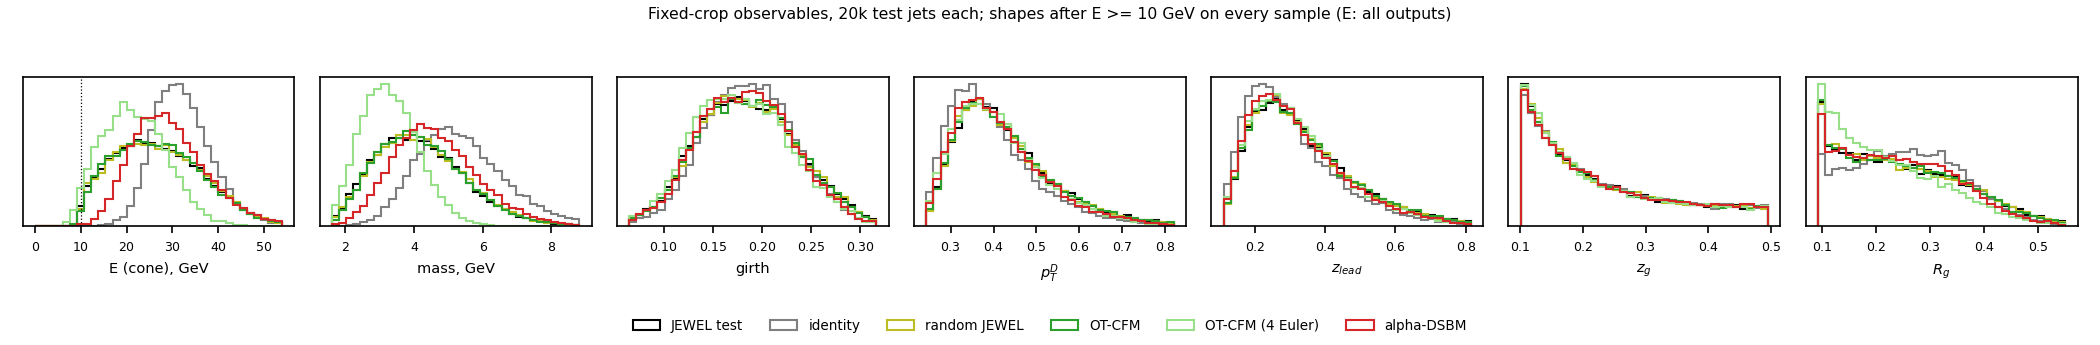
\includegraphics[width=0.99\textwidth]{tr_marginals.png}
\end{center}
\vspace{-1.1em}
\begin{columns}[T]
\column{0.64\textwidth}
\scriptsize
\setlength{\tabcolsep}{2pt}
\begin{tabular}{lrrrrrrrr}
\toprule
 & pass & $E$ & mass & girth & $p_T^D$ & $z_\mathrm{lead}$ & $z_g$ & $R_g$ \\
\midrule
JEWEL ref & 1.000 & 0.011 & 0.014 & 0.009 & 0.018 & 0.019 & 0.012 & 0.008 \\
random JEWEL & 1.000 & 0.019$^\circ$ & 0.024$^\circ$ & 0.011$^\circ$ & 0.010$^\circ$ & 0.011$^\circ$ & 0.005$^\circ$ & 0.010$^\circ$ \\
identity & 1.000 & 0.546 & 0.881 & 0.105 & 0.264 & 0.232 & 0.034$^\circ$ & 0.158 \\
\midrule
\ot{} & 0.995 & \textbf{0.025}$^\circ$ & \textbf{0.021}$^\circ$ & \textbf{0.012}$^\circ$ & \textbf{0.010}$^\circ$ & \textbf{0.008}$^\circ$ & 0.017$^\circ$ & \textbf{0.012}$^\circ$ \\
\ot{}, 4 Euler$^\ast$ & 0.974 & \textbf{0.510} & \textbf{0.678} & 0.129 & \textbf{0.125} & \textbf{0.099} & 0.010$^\circ$ & 0.249 \\
\dsbm{} & 0.999 & \textbf{0.256} & \textbf{0.325} & \textbf{0.056} & \textbf{0.112} & \textbf{0.099} & 0.036$^\circ$ & \textbf{0.073} \\
\bottomrule
\end{tabular}
\\[0.2em]
\snote{W1/$\sigma$ to 20k held-out JEWEL test jets (bootstrap sd 0.004-0.011); every sample cut at cone $E \ge$
10 GeV, pass = share of outputs kept (JEWEL: 1 by construction). \textbf{Bold}: below the identity by $>$ 3 sd;
$^\circ$: within 3 sd of the JEWEL-ref floor. $^\ast$speed readout only.}
\column{0.36\textwidth}
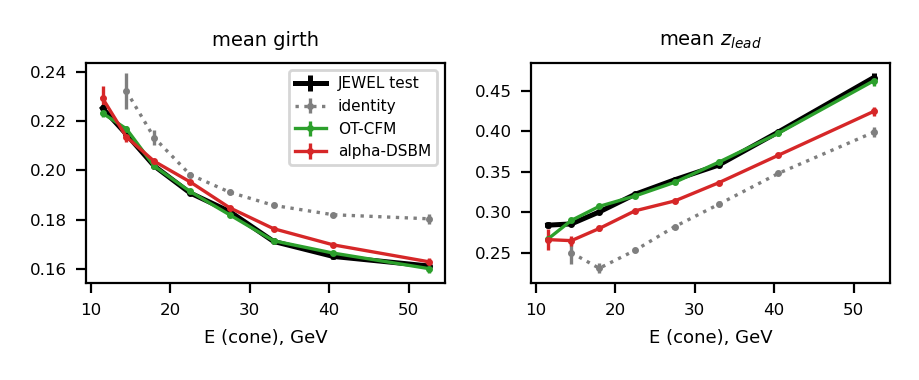
\includegraphics[width=\textwidth]{tr_profiles.png}\\[-0.3em]
\scriptsize
\begin{itemize}\setlength\itemsep{0.0em}
\item \textbf{joint}, W1/$\sigma$ in $E$ bins 10-20 / 20-30 / 30-60 GeV: girth \ot{} 0.023 / 0.012 / 0.020,
  $z_\mathrm{lead}$ 0.030 / 0.025 / 0.016 (floor 0.02-0.04; identity 0.16-0.47; \dsbm{} 0.07-0.18)
\item \textbf{refound} anti-$k_T$ jets ($p_T \ge$ 10 GeV): \ot{} within the floor in all 7 (pass 0.978,
  JEWEL 0.976); \dsbm{} 0.03-0.34
\item \dsbm{} closes 51-64\% of the identity's gap; 4 Euler steps barely move $E$
\end{itemize}
\end{columns}
\end{frame}

% ---------------------------------------------------------------- T3
\begin{frame}{Each output keeps its input's layout; the energy change follows the spectra}
\vspace{-0.6em}
\begin{columns}[T]
\column{0.5\textwidth}
\scriptsize
\setlength{\tabcolsep}{3pt}
\begin{tabular}{lrrrrrr}
\toprule
 & \multicolumn{5}{c}{correlation, input vs output} & own input \\
 & $E$ & girth & mass & core & lead & preferred \\
\midrule
identity & 1.00 & 1.00 & 1.00 & 1.00 & 1.00 & 1.000 \\
random JEWEL & 0.01 & -0.00 & 0.01 & -0.00 & -0.00 & 0.498 \\
\ot{} & 0.94 & 0.99 & 0.91 & 0.99 & 0.92 & 1.000 \\
\ot{}, 4 Euler$^\ast$ & 0.86 & 0.99 & 0.82 & 0.99 & 0.89 & 1.000 \\
\dsbm{} & 0.80 & 0.98 & 0.88 & 0.98 & 0.79 & 1.000 \\
\bottomrule
\end{tabular}
\\[0.1em]
\snote{20k test jets, no selection (bootstrap sd of a correlation $\le$ 0.003). Own input preferred: the output
is closer (normalised-shape EMD) to its input than to another test jet. These describe the maps, not errors.}
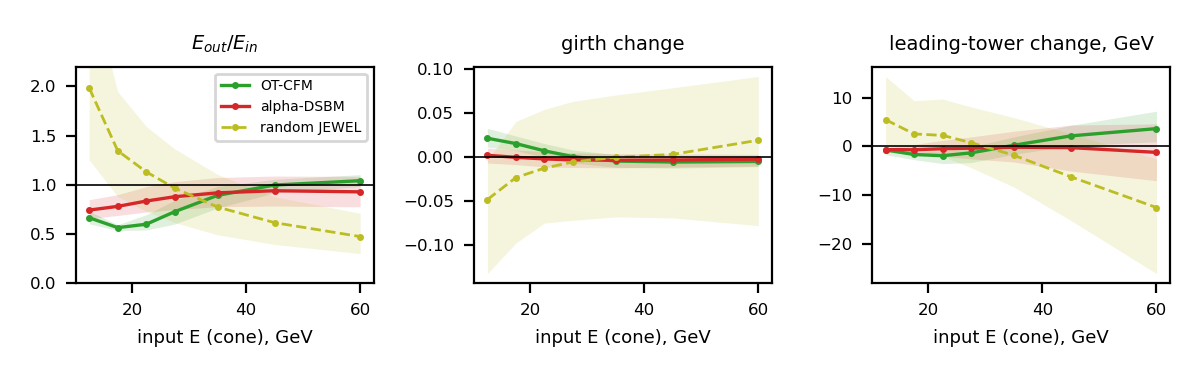
\includegraphics[width=\textwidth]{tr_changes_slide.png}\\[-0.3em]
\scriptsize
\begin{itemize}\setlength\itemsep{0.0em}
\item \ot{} $E_\mathrm{out}/E_\mathrm{in}$ (median): 0.60 at 20-25 GeV, 0.89 at 30-40, 1.00-1.04 above 40 GeV:
  the two samples' spectra (PYTHIA from 20 GeV, JEWEL from 10), not an energy-loss mechanism; hard jets get
  a harder core, as JEWEL's have. \dsbm{}: 0.84-0.94, flatter
\end{itemize}
\column{0.5\textwidth}
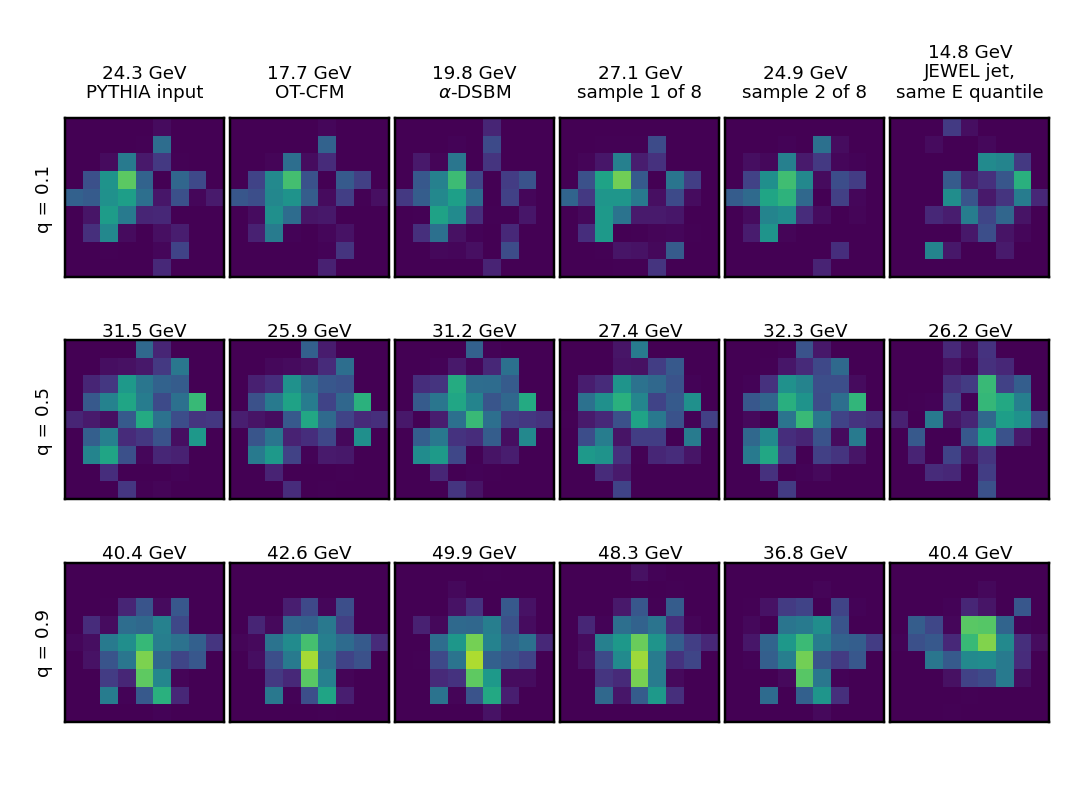
\includegraphics[width=\textwidth]{tr_displays_slide.png}\\[-0.2em]
\scriptsize
Fixed inputs (first 1000 test jets at cone-$E$ quantiles $q$), one output each; \dsbm{}: its output and 2 of
8 samples. Two samples of one jet differ more (shape EMD 0.068) than a sample differs from its input (0.056);
per-jet energy spread 0.37 $\sigma_E$: algorithmic variability, not a physical uncertainty.
\end{columns}
\end{frame}

% ---------------------------------------------------------------- T4
\begin{frame}{What the pilot establishes, what it does not, and cost}
\vspace{-0.7em}
\begin{columns}[T]
\column{0.57\textwidth}
\scriptsize
\setlength{\tabcolsep}{2.5pt}
\begin{tabular}{lrrrrrr}
\toprule
 & GPU h & updates & upd./s & overhead & NFE & ms/jet \\
\midrule
\ot{} & 2.00 & 122.7k & 17.0 & 10\% OT & 128 & 6.58 \\
\quad 4 Euler$^\ast$ & & & & & 4 & 0.21 \\
\dsbm{} pretrain & 0.50 & 26.1k & 14.5 & -- & & \\
\quad + refine & 1.50 & 8.8k & 1.62 & 89\% roll-out & 30 & 1.55 \\
\bottomrule
\end{tabular}
\\[0.1em]
\snote{One A6000 each; GPU h: training time, rollouts included; peak memory 3.5-3.8 GB; latency at batch
2000. Solver on validation:
\ot{} 32 vs 64 NFE moves a jet's energy by 8\% of its change (rule 1\%), 64 vs 128 1.6\%, 128 vs 256 0.5\%
$\Rightarrow$ 128. \dsbm{} 30 vs 60 steps, same noise: 0.55 GeV vs 6.0 between samples $\Rightarrow$ 30.}
\column{0.43\textwidth}
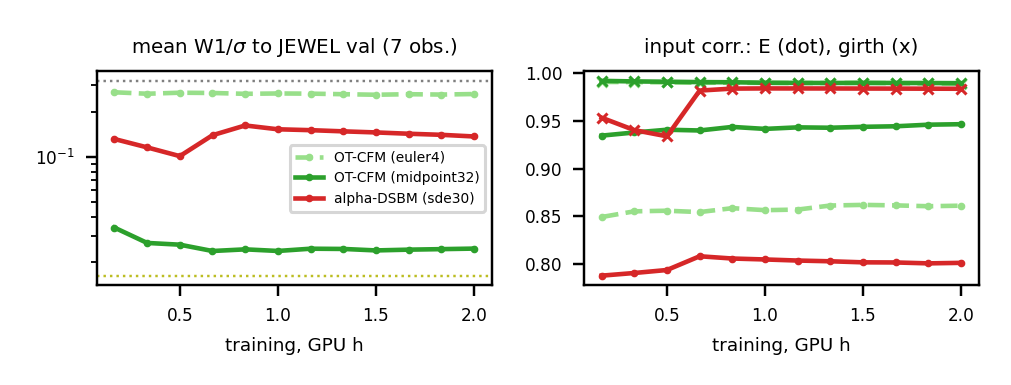
\includegraphics[width=\textwidth]{tr_curves_slide.png}\\[-0.3em]
\snote{Validation every 10 min (\ot{} at 32 NFE). \dsbm{}'s refinement worsened its pretrained distributions
(mean 0.10 $\to$ 0.14) while tightening the coupling; $E$ and mass still improving at 2 h.}
\end{columns}
\vspace{0.5em}
\scriptsize
\begin{columns}[T]
\column{0.5\textwidth}
\textbf{Measured} (seed 0, 20k held-out jets each)
\begin{itemize}\setlength\itemsep{0.0em}
\item \ot{}: all 7 fixed-crop and 7 refound-jet distributions and both $E$-shape joints within the
  JEWEL-vs-JEWEL floor; input correlations 0.91-0.99; no soft floor or flattening above 0.01 GeV
  (pre-registered reading: useful)
\item \dsbm{} ($\varepsilon$ 0.25): toward JEWEL in 6 of 7 and both joints, but 5-23$\times$ the floor;
  large per-jet randomness
\item below 0.01 GeV both fill 10-15 of JEWEL's 20 empty cone towers with $\sim$0.002 GeV (0.1\% of $E$):
  a limit of $\log(E + 0.1)$
\end{itemize}
\column{0.5\textwidth}
\textbf{Not established}
\begin{itemize}\setlength\itemsep{0.0em}
\item a per-jet medium modification: no truth exists; the map is OT's least change in $\log E$, and its high
  input correlation is partly by construction
\item physics in the energy change: it follows the samples' spectra, in a crop without out-of-cone energy
\item robustness: one seed; \dsbm{}'s limit at a larger budget
\end{itemize}
\textbf{One follow-up:} \ot{} seeds 1 and 2 (same data, cost, budget, 128 NFE): is the \emph{per-jet} map
reproducible, not only its distributions?
\end{columns}
\end{frame}
